% Provenance (never printed): see sources/outline_sources.md (Year 2: effusive and explosive
% eruptions, eruptive styles, eruption columns, pyroclastic deposits, explosivity index,
% volcano monitoring).
% Curves from figdata/bachelor-2/eruptions.py (closed-system gas fraction, Cotopaxi Layer 5
% thinning, GVP frequency-size law, column height fits, Mogi uplift); exercise and problem
% values in the Book 4 scratch calculators calc/ch06.py and calc/ch06pb.py.
\chapter{火山喷发}\label{ch:b2:eruptive-styles}

1991 年 6 月 15 日，菲律宾的皮纳图博火山喷出了超过
五立方千米的物质；火山灰云升至
\qty{35}{km}，山顶崩塌成一个直径为\qty{2.5}{km}的\omterm{def:b2:eruptive-styles:caldera}{破火山口}，而
它注入平流层的 2000 万吨二氧化硫使
整个地球降温约半度，持续两年。一周前，最先
抵达地表的\omterm{def:b2:magma-emplacement:magma}{岩浆}却并未如此：它在上升途中已失去大部分
气体，只是缓缓溢出，形成\omterm{def:b2:eruptive-styles:dome}{熔岩穹丘}。在夏威夷的基拉韦厄火山，
Pu`u~`\=O`\=o 喷发共喷出 \qty{4.4}{km^3} 熔岩，体积相当，
历时三十五年，以喷泉和熔岩流的形式摧毁了 215 座建筑，
却从未形成高耸的火山灰柱。同一个地球，同样的物理规律，三种行为，其区别在于
\omterm{def:b2:magma-emplacement:magma}{岩浆}携带多少气体、这些气体能否悄然
从熔体中逸出，以及\omterm{def:b2:magma-emplacement:magma}{岩浆}上升的速度有多快。本章追踪一次喷发，
从通道中的气泡，到喷口上方的\omterm{def:b2:eruptive-styles:column}{喷发柱}，再到
它留下的堆积物；随后测量喷发、统计次数，并监测火山，以寻找
即将喷发的迹象。
% ledger: usgs:pinatubo-1991, usgs:puuoo

\begin{recall}
\textbf{来自中学分册}：火山、喷口与火山口、其下方的\omterm{def:b2:magma-emplacement:magma}{岩浆}
房、熔岩和火山灰。\textbf{来自
\cref{ch:b2:magma-emplacement}}：\omterm{def:b2:magma-emplacement:volatiles}{岩浆挥发分}及其在低于
饱和压强时的出溶，水溶解度的平方根定律 $w = s\sqrt p$，其中
玄武岩取 $s \approx 0.34$（单位为每 $\sqrt{\unit{MPa}}$ 的百分比），
流纹岩取 $0.44$；熔体黏度相差十个数量级。
\textbf{来自物理教材}：理想气体状态方程 $pV = nRT$；浮力；
量纲分析，它由给定量构造唯一的组合，
其量纲与答案相同；抛体射程 $v^2\sin 2\theta/g$
（不计空气阻力）。\textbf{来自数学教材}：泊松过程，
其中独立事件以恒定速率 $\lambda$ 发生，
在时间 $t$ 内至少发生一次的概率为 $1 - e^{-\lambda t}$；最小二乘直线。
来自本科一年级分册：地震及其震级。
\end{recall}

\section{溢流式还是爆炸式}

\begin{definition}[溢流式与爆炸式喷发、岩浆破碎]\label{def:b2:eruptive-styles:regimes}
称\emph{溢流式喷发}\index{溢流式喷发}为以熔岩溢出为主的
喷发，熔岩以连续液体的形式离开喷口流走。
称\emph{爆炸式喷发}\index{爆炸式喷发}为主要产生
碎屑、火山灰、浮石和弹道碎屑，由膨胀的气体携带。
\emph{岩浆破碎}\index{岩浆破碎}是含气泡的连续熔体破裂为
携带熔体液滴与碎片的连续气相；
它使溢流式喷发转变为爆炸式喷发。
\end{definition}
% ledger: usgs:glossary-ch6, cassidy18:fragmentation

驱动这一转变的是气体。从深部上升的\omterm{def:b2:magma-emplacement:magma}{岩浆}携带
溶解的水和二氧化碳；低于其饱和压强时，挥发分
以气泡的形式出溶，气泡随压强降低而膨胀。
若气体留在熔体中，不久便会充满大部分体积。

\begin{proposition}[封闭系统脱气中的气体体积分数]\label{prop:b2:eruptive-styles:gas}
设\omterm{def:b2:magma-emplacement:magma}{岩浆}中水的质量分数为 $w_0$，溶解度 $w(p) =
s\sqrt p$，并假设出溶的水以温度为 $T$ 的理想
气体形式随熔体存在。低于饱和压强 $p_s = (w_0/s)^2$ 时，
1 千克\omterm{def:b2:magma-emplacement:magma}{岩浆}含有 $x = w_0 - s\sqrt p$ 千克水汽，
气体的体积分数为
\[
\phi(p) = \frac{V_g}{V_g + V_m}, \qquad V_g = \frac{x\,RT}{M p}, \qquad
V_m = \frac{1 - x}{\rho_m},
\]
其中 $M = \qty{0.018}{kg/mol}$ 为水的摩尔质量，$\rho_m$ 为
熔体的密度。
\end{proposition}

\begin{proof}
高于 $p_s$ 时，熔体可容纳全部水分，不存在气体。低于 $p_s$ 时，
熔体仅保留溶解度 $s\sqrt p$，因此每千克\omterm{def:b2:magma-emplacement:magma}{岩浆}中质量为 $x = w_0 - s\sqrt p$
的部分为水汽。该水汽为 $x/M$ 摩尔，占据体积 $xRT/(Mp)$，
由理想气体状态方程给出。其余 $1 - x$ 千克熔体占据体积 $(1 - x)/\rho_m$。
体积分数由此得出。
\end{proof}
% ledger: moore98:h2o

由于 $V_g$ 随 $1/p$ 增大，泡沫在近地表处膨胀最快。下
图追踪一条含 \qty{5}{\percent} 水的流纹岩与一条
含 \qty{1}{\percent} 水的玄武岩。流纹岩在 \qty{127}{MPa} 处饱和，约
位于地下 \qty{5}{km} 处；在 \qty{10}{MPa} 时，其气体已占
体积的 \qty{82}{\percent}。在一个已发表的导管流动模型中，\omterm{def:b2:magma-emplacement:magma}{岩浆}在
气体占其体积的 \qty{85}{\percent} 时破碎，流纹岩在
\qty{8.2}{MPa} 处达到此水平，约位于喷口下方 \qty{330}{m}，取压强梯度为
\qty{0.025}{MPa/m}。玄武岩仅在 \qty{8.7}{MPa} 时饱和，并达到
相同泡沫状态时压强为 \qty{1.8}{MPa}，距地表一百米以内。
% ledger: cassidy18:fragmentation, cassidy18:ascent

\begin{omfigure}
\centering
\begin{tikzpicture}
\begin{axis}[omrecord, width=0.82\linewidth, height=5.6cm, xmode=log,
  xmin=0.01, xmax=200, ymin=0, ymax=1,
  xlabel={压强 (\unit{MPa})}, ylabel={气相体积分数 $\phi$},
  legend pos=south west, legend style={font=\scriptsize},
  tick label style={font=\scriptsize}, label style={font=\small}]
\addplot[very thick, red!70!black] table[x=p_MPa, y=rhyolite] {figdata/out/bachelor-2-eruptions-gas.dat};
\addlegendentry{流纹岩，\qty{5}{\percent} H$_2$O，\qty{850}{\celsius}}
\addplot[very thick, black, dashed] table[x=p_MPa, y=basalt] {figdata/out/bachelor-2-eruptions-gas.dat};
\addlegendentry{玄武岩，\qty{1}{\percent} H$_2$O，\qty{1200}{\celsius}}
\draw[densely dotted, thick, gray] (axis cs:0.01,0.85) -- (axis cs:200,0.85);
\node[anchor=north west, font=\scriptsize, inner sep=1pt] at (axis cs:0.012,0.835) {导管模型中的岩浆破碎};
\end{axis}
\end{tikzpicture}
\par\smallskip{\small 出溶水汽的体积分数与压强的关系
（封闭系统脱气，见\cref{prop:b2:eruptive-styles:gas}），并采用
\cref{ch:b2:magma-emplacement}中的溶解度定律。压强向左降低，\omterm{def:b2:magma-emplacement:magma}{岩浆}随之
上升；虚线标出一个已发表的导管模型中
\omterm{def:b2:eruptive-styles:regimes}{岩浆破碎}时的气体体积分数。}
\end{omfigure}
% ledger: moore98:h2o, cassidy18:fragmentation

所以玄武岩若让气体留在其中，同样会破碎；在夏威夷式熔岩喷泉中，
喷口附近正是如此。大多数玄武质喷发之所以温和，
关键在于气体不必留在\omterm{def:b2:magma-emplacement:magma}{岩浆}中。在低黏度的熔体中，气泡穿过
液体上升、合并并逸出；一旦气泡连接成可渗透的网络，
实验中当气体体积分数介于 \qty{30}{\percent} 与 \qty{78}{\percent} 之间时即会发生，
气体便穿过管壁与喷口逸出，而不带走
熔体：\omterm{def:b2:magma-emplacement:magma}{岩浆}在开口系统中脱气，以熔岩的形式
到达地表。高黏度的\omterm{def:b2:magma-emplacement:magma}{岩浆}则保留气泡，并转而碎裂；熔体
在拉伸速度超过其流动速度时，会像玻璃一样断裂。上升速率
与成分同样决定两者之间的区别：在许多次喷发中，\omterm{def:b2:eruptive-styles:regimes}{溢流式喷发}
对应的减压速率约为 \qty{0.0001}{MPa/s}，\omterm{def:b2:eruptive-styles:regimes}{爆炸式喷发}
对应的速率约为 \qty{1}{MPa/s}，熔体黏度改变半个
对数单位（约为三倍）便足以使喷发从一种
模式转为另一种。皮纳图博火山的第一座\omterm{def:b2:eruptive-styles:dome}{熔岩穹丘}与一周后的
高潮式喷发来自同一\omterm{def:b2:magma-emplacement:magma}{岩浆}：第一批\omterm{def:b2:magma-emplacement:magma}{岩浆}有时间排出气体，后一批则没有。
% ledger: cassidy18:fragmentation, cassidy18:ascent, usgs:pinatubo-1991

外部水的作用与\omterm{def:b2:magma-emplacement:magma}{岩浆}自身的气体相同。地下水、湖泊或
与\omterm{def:b2:magma-emplacement:magma}{岩浆}接触的海水会瞬间汽化，过热水的膨胀
会使\omterm{def:b2:eruptive-styles:regimes}{岩浆破碎}：实验表明，超过 \qty{30}{\percent} 的
可用热量可转化为机械能。即便\omterm{def:b2:magma-emplacement:magma}{岩浆}中气体很少，
也可能因此发生\omterm{def:b2:eruptive-styles:regimes}{爆炸式喷发}。
% ledger: cassidy18:fragmentation

\section{喷发类型}

火山学家以经典实例为喷发命名。这些名称描述喷发的外观，
彼此之间并无截然界线；同一次喷发常会经历
多种类型。

\begin{definition}[喷发类型]\label{def:b2:eruptive-styles:styles}
按爆炸性由弱到强排列，以下为由\omterm{def:b2:magma-emplacement:magma}{岩浆}自身气体驱动的喷发：
\begin{itemize}
\item \emph{夏威夷式喷发}\index{夏威夷式喷发}产生由流动性极强的玄武质熔岩组成的喷泉，
喷高数十至数百米，并形成熔岩流；
\item \emph{斯特龙博利式喷发}\index{斯特龙博利式喷发}是一系列
离散的爆发，抛出炽热的玄武质至玄武安山质\omterm{def:b2:magma-emplacement:magma}{岩浆}团，
高达约一百米，且不形成持续的
\omterm{def:b2:eruptive-styles:column}{喷发柱}；
\item \emph{武尔卡诺式喷发}\index{武尔卡诺式喷发}是短暂而猛烈的爆炸，
由积聚在已固结熔岩塞之下的气体引发，并将其炸裂，
抛出岩块与深色的细灰柱，通常来自
中性\omterm{def:b2:magma-emplacement:magma}{岩浆}；
\item \emph{普林尼式喷发}\index{普林尼式喷发}是持续的气体与碎屑喷射，
碎裂的、通常为硅质的\omterm{def:b2:magma-emplacement:magma}{岩浆}，形成升入
平流层、持续数小时至数天的\omterm{def:b2:eruptive-styles:column}{喷发柱}，并
在数千平方千米范围内铺洒一层浮石与火山灰。
\end{itemize}
外部水驱动碎裂时，\emph{射汽岩浆
喷发}\index{射汽岩浆喷发}喷出蒸汽与
新鲜\omterm{def:b2:magma-emplacement:magma}{岩浆}碎片；而\emph{蒸汽喷发}\index{蒸汽喷发}是
由\omterm{def:b2:magma-emplacement:magma}{岩浆}或热岩加热的地下水或地表水驱动的蒸汽爆炸，
只喷出蒸汽与较老岩石的碎片，不含新鲜\omterm{def:b2:magma-emplacement:magma}{岩浆}。
\end{definition}
% ledger: nps:styles, usgs:glossary-ch6

每种喷发类型都有其典型实例。基拉韦厄火山上的 Pu`u~`\=O`\=o，
在其三十五年、六十一次活动中大部分时间属于夏威夷式，喷泉通常喷高
\qtyrange{10}{100}{m}，偶尔超过 \qty{500}{m}。斯特龙博利火山
被誉为“地中海的灯塔”，其名称已用于命名那些堆积成
火山渣锥的爆发。阿拉斯加的 Trident 火山曾断续遭受武尔卡诺式爆炸，
发生于 1953 年至 1974 年间。公元 79 年的维苏威火山由小普林尼记述，因此
其名称被用于命名\omterm{def:b2:eruptive-styles:styles}{普林尼式喷发}；1980 年 5 月 18 日的圣海伦斯火山，以及
1912 年的 Novarupta 火山，其\omterm{def:b2:eruptive-styles:column}{喷发柱}在持续近三天的喷发中升至 \qty{30}{km} 以上，
均为近代的例子。
介于两者之间的情形，\omterm{def:b2:eruptive-styles:column}{喷发柱}高度约在 \qty{20}{km} 以下、持续但不稳定，
称为亚普林尼式。若有水参与，\omterm{def:b2:eruptive-styles:styles}{斯特龙博利式喷发}便转为苏尔特塞式，
其名称取自 1963 年冰岛海岸外苏尔特塞岛的喷发，并堆成低矮的凝灰环与火山口湖；
普林尼式则转为射汽普林尼式。皮纳图博火山在 1991 年 3 月与 4 月，
蒸汽爆炸于北侧山坡炸出三个火山口，比高潮式喷发早两个月：
它们属于\omterm{def:b2:eruptive-styles:styles}{蒸汽喷发}。
% ledger: nps:styles, usgs:puuoo, usgs:glossary-ch6, usgs:pinatubo-deposits

\begin{definition}[熔岩穹丘]\label{def:b2:eruptive-styles:dome}
\emph{熔岩穹丘}\index{熔岩穹丘}是由黏稠熔岩构成的陡坡土丘，
通常为英安岩或流纹岩，自喷口缓慢挤出，堆积于喷口之上，
而不向外流走。
\end{definition}
% ledger: usgs:glossary-ch6

黏稠\omterm{def:b2:magma-emplacement:magma}{岩浆}失去气体后便形成穹丘：1991 年 6 月皮纳图博火山喷出的第一批
\omterm{def:b2:magma-emplacement:magma}{岩浆}，以及圣海伦斯火山火山口内、于 1980 年至 1986 年间分十七次生长的
穹丘，高出火山口底部 \qty{267}{m}。
穹丘也可充当塞子，气体将在其下积聚，直至引发下一次武尔卡诺式爆炸；
其坍塌则可释放下方富气\omterm{def:b2:magma-emplacement:magma}{岩浆}上的压力。下
图展示了这一范围的两端。
% ledger: usgs:pinatubo-1991, usgs:msh-dome, cassidy18:fragmentation

\begin{omfigure}
\centering
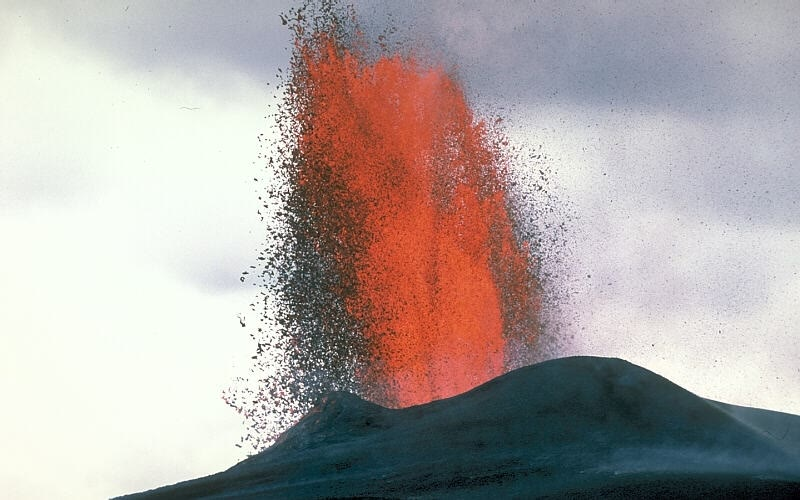
\includegraphics[height=4.3cm]{images/book4/b2-kilauea-fountain.jpg}\hfill
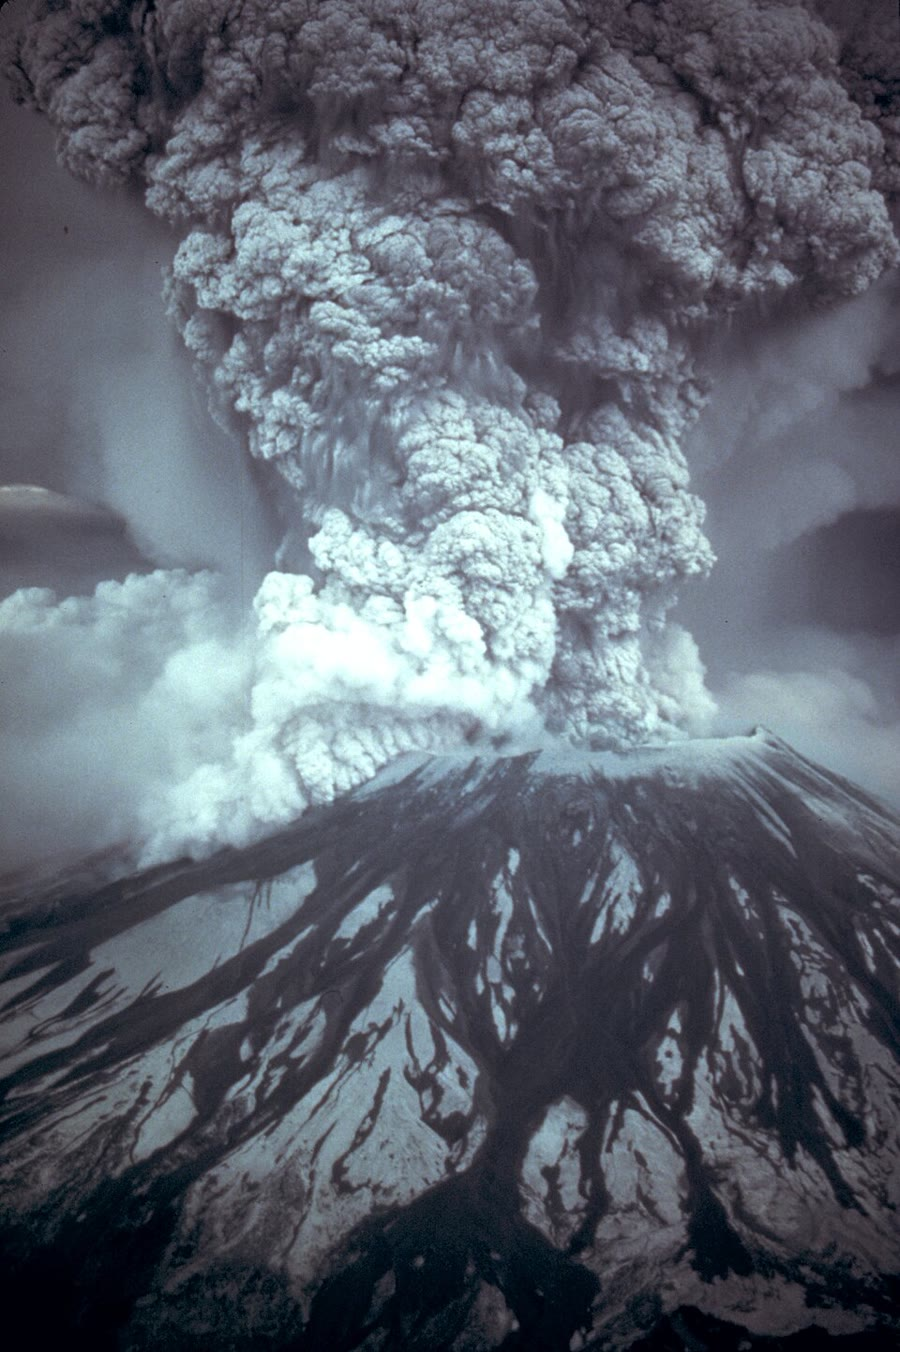
\includegraphics[height=4.3cm]{images/book4/b2-st-helens-column.jpg}\hfill
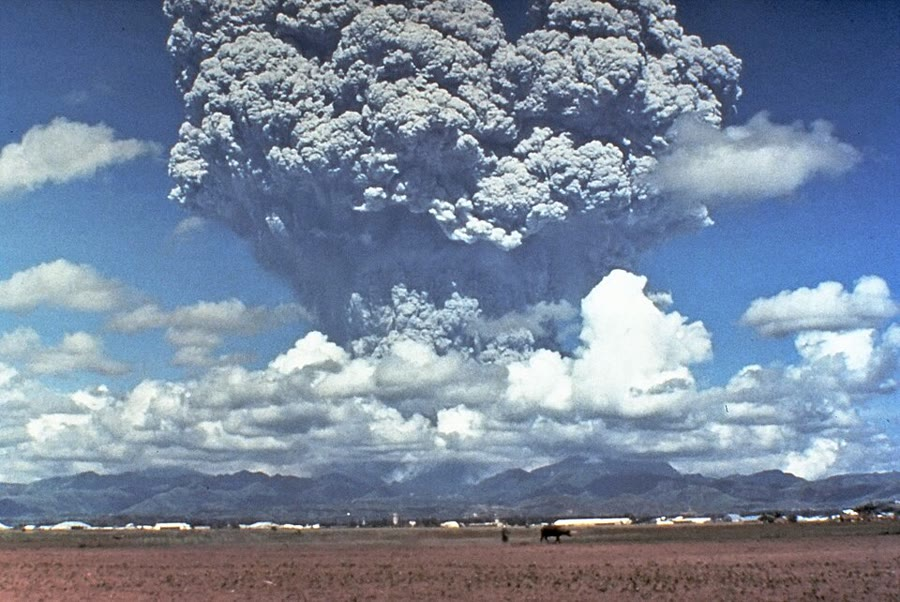
\includegraphics[height=4.3cm]{images/book4/b2-pinatubo-column.jpg}
\par\smallskip{\small 左：基拉韦厄火山 Pu`u~`\=O`\=o 火山锥上的夏威夷式喷泉，
1983 年 10 月（J.\,D.~Griggs，USGS）。中：圣海伦斯火山的\omterm{def:b2:eruptive-styles:styles}{普林尼式喷发}柱，
1980 年 5 月 18 日（Austin Post，USGS）。右：皮纳图博火山的\omterm{def:b2:eruptive-styles:column}{喷发柱}，
拍摄于 1991 年 6 月 12 日，即高潮式喷发前三天（Dave Harlow，USGS）。三张
照片均属公有领域。}
\end{omfigure}
% ledger: usgs:puuoo, usgs:msh-may18, usgs:pinatubo-1991

\section{喷发柱}

\begin{definition}[喷发柱]\label{def:b2:eruptive-styles:column}
\emph{喷发柱}\index{喷发柱}是爆炸性喷口之上上升的气体与
碎屑团。它分为三个部分：\emph{喷射区}，即
气体推进区，混合物以较快速度离开喷口，但密度大于空气，依靠动量上升；\emph{对流区}，其中混合物
卷入并加热了足够多的空气，密度变得低于
周围环境，依靠浮力上升；以及\emph{伞状区}，其
在柱体密度与大气密度相等的
高度处向两侧铺展。
\end{definition}
% ledger: usgs:glossary-ch6, nps:styles, aubry23:fits

\begin{omfigure}
\centering
\begin{tikzpicture}[x=1cm, y=1cm, font=\scriptsize]
% atmosphere and ground
\fill[blue!6] (-6.2,0) rectangle (6.2,6.4);
% volcano
\fill[brown!45, draw=brown!70!black] (-4.8,0) -- (-0.45,1.6) -- (0.45,1.6) -- (4.8,0) -- cycle;
% collapse branch (left): a density current hugging the flank
\fill[gray!55] (-0.45,1.6) -- (-0.7,2.35) .. controls (-1.1,2.25) and (-1.5,1.65) .. (-2.2,1.3)
  .. controls (-3.4,0.85) and (-4.6,0.42) .. (-5.9,0.28) -- (-5.9,0) -- (-4.8,0) -- cycle;
% jet
\fill[gray!70] (-0.45,1.6) -- (0.45,1.6) -- (0.75,2.5) -- (-0.75,2.5) -- cycle;
% convective column
\fill[gray!45] (-0.75,2.5) .. controls (-1.1,3.2) and (-1.0,3.8) .. (-1.4,4.2)
  -- (1.4,4.2) .. controls (1.0,3.8) and (1.1,3.2) .. (0.75,2.5) -- cycle;
% umbrella
\fill[gray!35] (-1.4,4.2) .. controls (-3,4.1) and (-5,4.2) .. (-5.8,4.45)
  .. controls (-5,4.9) and (-3,5.1) .. (0,5.25) .. controls (3,5.1) and (5,4.9) .. (5.8,4.45)
  .. controls (5,4.2) and (3,4.1) .. (1.4,4.2) -- cycle;
\draw[densely dashed, blue!60!black] (-6.2,4.4) -- (6.2,4.4);
% fallout from the far end of the umbrella, down to the ground
\foreach \x in {4.95,5.25,5.55} {\draw[gray!70, densely dotted, thick] (\x,4.3) -- (\x-0.1,0.02);}
\draw[gray, densely dotted] (0.45,1.6) -- (6.0,1.6);
\draw[<->] (6.0,1.6) -- (6.0,5.25) node[midway, right, align=left] {顶部 \\高度 \\$H$\\（火山口通道 \\以上）};
% labels
\node[anchor=north west, align=left, blue!60!black] at (-6.1,4.3) {中性浮力高度 \\（虚线）};
\draw (-0.95,3.3) -- (-1.8,3.05) node[left, align=right] {对流区：\\有浮力，卷入空气};
\draw (0.3,2.05) -- (2.0,2.35) node[right, align=left] {喷射区：靠动量上升，\\密度大于空气};
\draw (2.6,4.85) -- (3.2,5.75) node[right] {伞状云};
\node[anchor=east, align=right] at (4.8,1.25) {伞状云 \\降落的火山灰碎屑};
\draw (-3.4,0.7) -- (-3.9,1.5) node[above, align=center] {坍塌：火山碎屑 \\密度流};
\draw[-latex] (0,1.0) -- (0,1.55);
\node[anchor=north] at (0,1.0) {火山口通道};
\end{tikzpicture}
\par\smallskip{\small \omterm{def:b2:eruptive-styles:column}{喷发柱}结构（示意图，不按比例）。右侧
\omterm{def:b2:eruptive-styles:column}{喷发柱}穿过三个区域上升，伞状云铺展时降落\omterm{def:b2:eruptive-styles:tephra}{火山灰碎屑}；
左侧，部分喷射流未获得浮力，
坍塌成为\omterm{def:b2:eruptive-styles:pdc}{火山碎屑密度流}。}
\end{omfigure}

\omterm{def:b2:eruptive-styles:column}{喷发柱}能升多高，首先取决于它每秒带入的热量，
即质量喷发率~$Q$。借助量纲分析，
可以给出这一规律的形式。

\begin{proposition}[有浮力羽流的高度]\label{prop:b2:eruptive-styles:plume}
若稳定点源上方浮力羽流的顶部高度 $H$ 仅取决于
源的浮力通量 $F$（量纲 $\mathrm{m^4\,s^{-3}}$）以及
稳定层结大气的浮力频率 $N$（量纲
$\mathrm{s^{-1}}$），则
\[
H = c\,F^{1/4}N^{-3/4}
\]
其中 $c$ 为无量纲常数。由于 $F$ 与热通量成正比，
进而与质量喷发率成正比，于是在给定大气中 $H \propto Q^{1/4}$。
\end{proposition}

\begin{proof}
设 $H = c\,F^{\alpha}N^{\beta}$。比较长度量纲，得 $4\alpha = 1$；
比较时间量纲，得 $-3\alpha - \beta = 0$。于是 $\alpha = 1/4$，$\beta = -3/4$，且
除此之外，$F$ 与 $N$ 的其他组合都没有长度的量纲。
\end{proof}

常数 $c$ 取决于羽流卷入空气的快慢，羽流理论
用实验测定的卷入系数来处理，此处
在本阶段不加证明地承认。实际\omterm{def:b2:eruptive-styles:column}{喷发柱}并非静风大气中的稳定点源，因此
火山学家将该规律拟合到高度与质量喷发率
均已测得的喷发事件上。
% ledger: aubry23:fits

\begin{proposition}[喷发柱高度与质量喷发率]\label{prop:b2:eruptive-styles:mastin}
对于火山口通道以上的顶部高度 $H$（以千米计）与质量喷发率
$Q$（以千克每秒计），对记录完善的喷发事件进行汇总，得到
\[
H = 0.304\,Q^{0.241},
\]
另有一组包含 130 个事件的独立较大数据集，给出 $H = 0.345\,Q^{0.226}$。
离散程度很大：$H$ 的相对方均根误差
为 \qtyrange{53}{60}{\percent}。
\end{proposition}
\admitted
% ledger: aubry23:fits

两个指数都接近羽流理论中的 $1/4$。下图给出
两条拟合曲线，以及灰烬预报中心所用源参数所依据的
示例喷发。高 \qty{15}{km} 的\omterm{def:b2:eruptive-styles:column}{喷发柱}，如圣海伦斯火山
的喷发，需要 \qty{e7}{kg/s}，即每秒一万吨；高度加倍时
所需速率近十八倍。反过来，测得的高度
可以给出速率，但只能精确到数倍之内，因为 $Q$ 与 $H^4$
成正比（见\cref{exo:b2:eruptive-styles:3}）。火山学家用\emph{强度} $I =
\log_{10}Q + 3$，其中 $Q$ 的单位为千克每秒。
% ledger: mastin09:examples, aubry23:fits, brown14:record

\begin{omfigure}
\centering
\begin{tikzpicture}
\begin{axis}[omrecord, width=0.82\linewidth, height=6cm, xmode=log, ymode=log,
  xmin=1e3, xmax=1e9, ymin=1, ymax=60,
  xlabel={质量喷发率 $Q$（\unit{kg/s}）}, ylabel={火山口通道以上顶部高度（\unit{km}）},
  ytick={1,2,5,10,20,50}, yticklabels={1,2,5,10,20,50},
  legend pos=north west, legend style={font=\scriptsize},
  tick label style={font=\scriptsize}, label style={font=\small}]
\addplot[very thick, black] table[x=Q, y=mastin] {figdata/out/bachelor-2-eruptions-column.dat};
\addlegendentry{$H = 0.304\,Q^{0.241}$}
\addplot[thick, red!70!black, dashed] table[x=Q, y=aubry] {figdata/out/bachelor-2-eruptions-column.dat};
\addlegendentry{$H = 0.345\,Q^{0.226}$}
\addplot[only marks, mark=*, mark size=1.8pt, blue!70!black]
  table[x=Q, y=H] {figdata/out/bachelor-2-eruptions-column-data.dat};
\addlegendentry{示例喷发}
\begin{scope}[font=\tiny, inner sep=1.5pt]
\node[anchor=north west] at (axis cs:5e3,2) {埃特纳 2001};
\node[anchor=south east] at (axis cs:1e5,7) {塞罗内格罗 1992};
\node[anchor=north west] at (axis cs:2e5,5) {鲁阿佩胡 1996};
\node[anchor=east] at (axis cs:1e6,10) {富埃戈 1974};
\draw[gray] (axis cs:3e6,10) -- (axis cs:2e7,4.5) node[anchor=west, black] {苏弗里耶尔希尔斯};
\draw[gray] (axis cs:4e6,11) -- (axis cs:2e7,6.5) node[anchor=west, black] {斯珀尔 1992};
\node[anchor=south east] at (axis cs:1e7,15) {圣海伦斯 1980};
\node[anchor=south east, align=right] at (axis cs:1e8,25) {圣海伦斯 \\伴生熔结凝灰岩云};
\end{scope}
\end{axis}
\end{tikzpicture}
\par\smallskip{\small \omterm{def:b2:eruptive-styles:column}{喷发柱}在火山口通道以上的顶部高度，与
质量喷发率的关系：马斯廷等人（2009）的经验拟合，
奥布里等人（2023）对一组独立数据的拟合，以及
第一份汇编中的示例喷发（圣海伦斯火山的伴生\omterm{def:b2:eruptive-styles:pdc}{熔结凝灰岩}云
源自\omterm{def:b2:eruptive-styles:pdc}{火山碎屑流}，而非自火山口通道升起）。}
\end{omfigure}
% ledger: aubry23:fits, mastin09:examples

\omterm{def:b2:eruptive-styles:column}{喷发柱}也可能无法升起。喷射流离开火山口时比空气更致密；若在卷入足够空气、获得浮力之前
动量已耗尽（例如因气体含量下降），则\omterm{def:b2:eruptive-styles:column}{喷发柱}坍塌，混合物
便沿山坡以炽热而致密的流动形式倾泻而下。\omterm{def:b2:eruptive-styles:styles}{普林尼式喷发}柱可以
这样坍塌，在皮纳图博火山，
1991 年的\omterm{def:b2:eruptive-styles:pdc}{火山碎屑流}将山谷填埋，
沉积物厚达 \qty{200}{m}。
% ledger: nps:styles, usgs:pinatubo-deposits

\section{火山碎屑产物}

\begin{definition}[火山灰碎屑与火山碎屑]\label{def:b2:eruptive-styles:tephra}
一个\emph{火山碎屑}\index{火山碎屑}是\omterm{def:b2:magma-emplacement:magma}{岩浆}或其周围岩石
经爆炸性破碎而形成的碎片。\emph{火山灰碎屑}\index{火山灰碎屑}是
所有被抛入空中的火山碎屑的总称，不论其大小。
按粒径，细于 \qty{2}{mm} 的火山碎屑构成火山灰；
粒径为 \qtyrange{2}{64}{mm} 的是\emph{火山砾}\index{火山砾}；粒径大于
\qty{64}{mm} 的，若喷出时为固态且棱角分明，则称为火山块；
若喷出时全部或部分为熔融态，则称为\emph{火山弹}\index{火山弹}，
其在飞行中呈圆形或纺锤形。
\end{definition}
% ledger: nps:pyroclast-sizes, usgs:glossary-ch6

\omterm{def:b2:eruptive-styles:tephra}{火山灰碎屑}由伞状云与\omterm{def:b2:eruptive-styles:column}{喷发柱}落下，形成
覆盖陆地的降落沉积：近火山口处厚，远离则变薄、颗粒变细。其
厚度用\emph{等厚线}制图，等厚线即厚度相等的线，通常
随距离按指数规律递减。由于风把等厚线拉伸成
椭圆，距离最好以各等厚线
所围面积的平方根来度量。
% ledger: usgs:ash-props, biass19:layer5

\begin{proposition}[指数变薄沉积的体积]\label{prop:b2:eruptive-styles:thinning}
若降落沉积的厚度随等厚线所围面积的平方根 $x = \sqrt A$
按 $T = T_0\,e^{-kx}$ 递减，则其总体积为
\[
V = \frac{2T_0}{k^2}.
\]
该体积的一半位于等厚线 $x_{1/2} = 1.678/k$ 以外。
\end{proposition}

\begin{proof}
在面积分别为 $A$ 与 $A + dA$ 的两条等厚线之间，沉积物的体积为 $T\,dA$，
且 $dA = 2x\,dx$。于是 $V = \int_0^\infty T_0e^{-kx}\,2x\,dx = 2T_0/k^2$，
此处用分部积分（$\int_0^\infty xe^{-kx}dx = 1/k^2$）。等厚线 $x$ 以内的体积
为 $\frac{2T_0}{k^2}[1 - (1 + kx)e^{-kx}]$，当 $(1 +
u)e^{-u} = 1/2$（$u = kx$）时，恰为总体积的一半，即 $u = 1.678$。
\end{proof}

实际沉积物会以两段或更多段斜率变薄：近火山口处陡，远处平缓，
原因是粗的\omterm{def:b2:eruptive-styles:tephra}{火山砾}迅速自\omterm{def:b2:eruptive-styles:column}{喷发柱}落下，而细的火山灰则随风漂移。
每一段分别拟合，
逐段积分。

\begin{method}[由等厚线求降落沉积的体积]\label{met:b2:eruptive-styles:volume}
对每条等厚线，以 $\ln T$ 对 $\sqrt A$ 作图，
并对每一段近似共线的点拟合直线。若分为两段，内段为 $T_0e^{-k_1x}$，
两直线交点 $X$ 之外为第二段，则体积为
\[
V = \frac{2T_0}{k_1^2} + 2T_0e^{-k_1X}\left[\frac{k_2X + 1}{k_2^2} -
\frac{k_1X + 1}{k_1^2}\right]
\]
（见\cref{exo:b2:eruptive-styles:10}）。将总体积换算为致密岩当量，即与无气泡\omterm{def:b2:magma-emplacement:magma}{岩浆}质量相同的体积，
换算式为 $V_{\mathrm{DRE}} = V\rho_{\mathrm{deposit}}/\rho_{\mathrm{magma}}$。
\end{method}
% ledger: biass19:layer5, brown14:record

下图将该方法应用于厄瓜多尔科托帕希火山
约 \num{1200} 年前喷出的一层火山渣降落沉积。两段直线拟合六条等厚线，
厚度半距离 $\ln 2/k$ 分别为 \qty{1.9}{km} 和 \qty{5.0}{km}（
已发表的研究拟合略有不同，得到 \qty{1.9}{km} 与
\qty{5.3}{km}），体积为 \qty{0.29}{km^3}，与该研究一致。其中超过
\qty{40}{\percent} 位于较薄的远端段，这正是远端火山灰
（易被侵蚀或从未被测绘）对总量影响如此之大的原因。新落的火山灰
体积密度为 \qtyrange{500}{1500}{kg/m^3}，远低于
\omterm{def:b2:magma-emplacement:magma}{岩浆}的密度，因此致密岩当量约为总体积的一半或更少。
% ledger: biass19:layer5, usgs:ash-props

\begin{omfigure}
\centering
\begin{tikzpicture}
\begin{axis}[omrecord, width=0.78\linewidth, height=5.6cm, ymode=log,
  xmin=0, xmax=30, ymin=2, ymax=2000,
  xlabel={$\sqrt{\text{等厚线所围面积}}$ (\unit{km})}, ylabel={厚度 (\unit{cm})},
  ytick={2,5,10,20,50,100,200,500,1000,2000}, yticklabels={2,5,10,20,50,100,200,500,1000,2000},
  legend pos=north east, legend style={font=\scriptsize},
  tick label style={font=\scriptsize}, label style={font=\small}]
\addplot[thick, black, restrict x to domain=0:12] table[x=sqrtA_km, y=seg1] {figdata/out/bachelor-2-eruptions-thin-fit.dat};
\addlegendentry{近端段，$k_1 = \qty{0.365}{km^{-1}}$}
\addplot[thick, red!70!black, dashed, restrict x to domain=5:30] table[x=sqrtA_km, y=seg2] {figdata/out/bachelor-2-eruptions-thin-fit.dat};
\addlegendentry{远端段，$k_2 = \qty{0.138}{km^{-1}}$}
\addplot[only marks, mark=*, mark size=2pt, blue!70!black] table[x=sqrtA_km, y=T_cm] {figdata/out/bachelor-2-eruptions-thin-data.dat};
\addlegendentry{等厚线}
\end{axis}
\end{tikzpicture}
\par\smallskip{\small 厄瓜多尔科托帕希火山第~5~层火山渣降落沉积的变薄情况，
约 \num{1200} 年前：比亚斯、博纳多纳与
霍顿（2019）给出的等厚线厚度，与各等厚线所围面积平方根的关系（
纵轴为对数刻度）。两段指数拟合分别对应两条
近端与四条远端等厚线，在 $\sqrt A = \qty{8.6}{km}$ 处相交；
积分后得到总体积为 \qty{0.29}{km^3}。}
\end{omfigure}
% ledger: biass19:layer5

不是所有\omterm{def:b2:eruptive-styles:tephra}{火山碎屑}都从天而降。当\omterm{def:b2:eruptive-styles:column}{喷发柱}坍塌、\omterm{def:b2:eruptive-styles:dome}{熔岩穹丘}崩裂，或
侧向爆发撕裂火山的一侧时，炽热的混合物便沿
地面流动。

\begin{definition}[火山碎屑密度流]\label{def:b2:eruptive-styles:pdc}
一个\emph{火山碎屑密度流}\index{火山碎屑密度流}是一种贴近地面流动的
热气体与\omterm{def:b2:eruptive-styles:tephra}{火山碎屑}的混合物，沿坡向下或向外流动，
因其比空气致密。一个\emph{火山碎屑流}\index{火山碎屑流}
是由岩石碎片、火山灰和气体组成的集中流，通常温度为
\qtyrange{200}{700}{\celsius}，速度可达每秒数十米；而
\emph{火山碎屑涌流}\index{火山碎屑涌流}则是较稀薄的火山灰、岩石与气体云，
温度达数百摄氏度，其速度可与飓风
风速相当。\emph{熔结凝灰岩}\index{熔结凝灰岩}是由\omterm{def:b2:eruptive-styles:tephra}{火山碎屑}密度流沉积形成的岩石，
可能借自身余热而发生熔结。
\end{definition}
% ledger: usgs:glossary-ch6

1980 年 5 月 18 日，圣海伦斯火山北翼发生崩塌，形成有记录以来
规模最大的滑坡（体积约 \qty{2.8}{km^3}），使\omterm{def:b2:magma-emplacement:magma}{岩浆}失去覆盖，并
释放一次侧向爆炸，横扫约 \qty{600}{km^2} 的区域，速度可达
\qty{480}{km/h}；随后，温度至少 \qty{700}{\celsius} 的\omterm{def:b2:eruptive-styles:pdc}{火山碎屑流}抵达
距火山口 \qty{8}{km} 处。1991 年皮纳图博火山的\omterm{def:b2:eruptive-styles:pdc}{火山碎屑流}，
五年后其内部温度仍高达 \qty{500}{\celsius}。
% ledger: usgs:msh-may18, usgs:msh-flows, usgs:msh-reach, usgs:pinatubo-deposits

\begin{definition}[火山泥流]\label{def:b2:eruptive-styles:lahar}
一个\emph{火山泥流}\index{火山泥流}是快速流动的水与\omterm{def:b2:eruptive-styles:tephra}{火山碎屑}的混合物，
沿河谷向下流动，其稠度从浑水到湿混凝土不等。
火山泥流形成于\omterm{def:b2:eruptive-styles:pdc}{火山碎屑流}融化积雪与冰川之时、
大雨落在松散火山堆积物上之时、被火山堆积物堵塞的湖泊溃决之时，
或由碎屑崩落引发。
\end{definition}
% ledger: usgs:glossary-ch6

\omterm{def:b2:eruptive-styles:lahar}{火山泥流}的持续时间常长于喷发本身。在皮纳图博火山周围，季风与台风带来的降雨，
使 1991 年的火山灰多年间不断转化为\omterm{def:b2:eruptive-styles:lahar}{火山泥流}，
造成的破坏甚至超过喷发本身。
% ledger: usgs:pinatubo-lahars

\begin{definition}[破火山口]\label{def:b2:eruptive-styles:caldera}
一个\emph{破火山口}\index{破火山口}是一种大型盆状火山洼地，
直径为 \qtyrange{2}{50}{km}，远大于其内任何火山口通道，
由地面塌陷进入一个浅层\omterm{def:b2:magma-emplacement:magma}{岩浆}储库而形成，该储库已被一次喷发
部分排空。
\end{definition}
% ledger: usgs:glossary-ch6

皮纳图博与诺瓦鲁普塔火山的\omterm{def:b2:eruptive-styles:caldera}{破火山口}直径均约为 \qty{2.5}{km}，
处于该范围的较小一端。\omterm{def:b2:eruptive-styles:caldera}{破火山口}不同于火山口，后者更小，由爆炸挖掘形成。
% ledger: usgs:pinatubo-1991, nps:styles, usgs:glossary-ch6

\section{测定与计数喷发}

\begin{definition}[火山爆发指数]\label{def:b2:eruptive-styles:vei}
\emph{火山爆发指数}\index{火山爆发指数}（VEI）是
一个取值为 0 至 8 的整数，用以度量喷发规模，主要依据\omterm{def:b2:eruptive-styles:tephra}{火山碎屑}的
堆积总体积：体积小于 \qty{e4}{m^3} 为 VEI~0，体积至
\qty{e6}{m^3} 为 VEI~1，此后体积每增大十倍，指数升高一级，直至
超过 \qty{e12}{m^3}（即 \qty{1000}{km^3}）时为 VEI~8。\omterm{def:b2:eruptive-styles:column}{喷发柱}高度与喷发的描述，
在体积未知时采用。非爆炸性喷发的 VEI~0，
无论其熔岩体积多大。
\end{definition}
% ledger: usgs:vei-criteria, usgs:msh-comparisons

\begin{table}[ht]
\centering
\small
\begin{tabular}{llll}
\hline
VEI & 堆积体积 (\unit{m^3}) & \omterm{def:b2:eruptive-styles:column}{喷发柱}高度 (\unit{km}) & 常见类型 \\
\hline
0 & $< 10^{4}$ & $< 0.1$ & 夏威夷式 \\
1 & $10^{4}$--$10^{6}$ & 0.1--1 & 夏威夷式、斯特龙博利式 \\
2 & $10^{6}$--$10^{7}$ & 1--5 & 斯特龙博利式、武尔卡诺式 \\
3 & $10^{7}$--$10^{8}$ & 3--15 & 武尔卡诺式 \\
4 & $10^{8}$--$10^{9}$ & 10--25 & 武尔卡诺式、普林尼式 \\
5 & $10^{9}$--$10^{10}$ & $> 25$ & 普林尼式 \\
6 & $10^{10}$--$10^{11}$ & $> 25$ & 普林尼式 \\
7 & $10^{11}$--$10^{12}$ & $> 25$ & 普林尼式 \\
8 & $> 10^{12}$ & $> 25$ & 普林尼式 \\
\hline
\end{tabular}
\caption{\omterm{def:b2:eruptive-styles:vei}{火山爆发指数}的判据（依据 Newhall 与 Self，1982）。}
\label{tab:b2:eruptive-styles:vei}
\end{table}
% ledger: usgs:vei-criteria

该指数与地震震级一样是对数的，但分级更粗。
1980 年的圣海伦斯火山喷出 \qty{1.3}{km^3} 火山灰，被定为 VEI~5，“但仅勉强达到”；
1991 年的皮纳图博火山定为 VEI~6；1815 年的坦博拉火山喷出的火山灰
为圣海伦斯火山的三十至八十倍，定为 VEI~7，是有历史记载以来规模最大的\omterm{def:b2:eruptive-styles:regimes}{爆炸式喷发}。
定量研究中，火山学家更偏好使用
\emph{震级}$M = \log_{10}m - 7$，其中 $m$ 为喷出物质的质量（单位为千克），
该式避开了堆积物的体积密度，
速率则采用前文定义的强度。
% ledger: usgs:msh-1980-ash, usgs:msh-comparisons, data:b4-gvp-eruptions, brown14:record

小规模喷发频繁，大规模喷发罕见。全球全新世喷发目录
使这一关系得以定量化，但需考虑其中的空位：
一次喷发只有被人记录或其堆积物被发现，才会进入目录，
远离观测者的小规模喷发，或距今超过数百年的喷发，往往被遗漏。
大规模喷发的记录完整期长于小规模喷发。在下图左侧，
各级喷发自 1500 年以来的累积数随时间增加；
若记录完整且速率恒定，则应沿对角线分布。
VEI~3 及以上的喷发大多集中在最近一个世纪，
因为早期的大多数喷发未被记录；VEI~6 的记录
则接近对角线。
% ledger: data:b4-gvp-eruptions, brown14:record

\begin{dated}{2026}
全球火山活动计划目录列出 \num{7747} 次经确认的全新世喷发，
均标有 VEI。自各统计时段起点计至 2024 年底，
1950 年以来 VEI~3 及以上的喷发有 399 次，1900 年以来 VEI~4 及以上的有 95 次，
1800 年以来 VEI~5 及以上的有 22 次，1500 年以来 VEI~6 及以上的有 8 次
（最近一次为 1991 年的皮纳图博火山）。自公元 1000 年以来，仅记录到两次 VEI~7 的喷发：
1257 年的林贾尼火山，以及始于 1812 年、于
1815 年达到高潮的坦博拉火山。
\end{dated}
% ledger: data:b4-gvp-eruptions, usgs:msh-comparisons

\begin{proposition}[喷发频率–规模定律]\label{prop:b2:eruptive-styles:frequency}
设 $\lambda_v$ 为地球上每年 VEI $\ge v$ 的喷发次数的均值，
每个值均在其记录接近完整的时段内估计（对 $v = 3$ 取 1950 年以来，
对 $v = 4$ 取 1900 年以来，对 $v = 5$ 取 1800 年以来，对 $v = 6$ 取 1500 年以来）。则由
最小二乘法可得
\[
\log_{10}\lambda_v = 3.28 - 0.85\,v .
\]
VEI 每升高一级，喷发频率约为其下一级的七分之一。
\end{proposition}
% ledger: data:b4-gvp-eruptions

该定律为经验性的，由四个数据点拟合而得，其指数取决于所选的
时段；它预测每 \num{470} 年发生一次 VEI~7 或更大的喷发，
与最近一千年中未用于拟合的两次喷发相近。由于
各次喷发近乎彼此独立，它们表现为泊松过程，
则 VEI $\ge v$ 的喷发在 $t$ 年内至少发生一次的概率为
$1 - e^{-\lambda_vt}$（周末问题）。
% ledger: data:b4-gvp-eruptions

\begin{omfigure}
\centering
\begin{tikzpicture}
\begin{axis}[omrecord, name=cum, width=0.47\linewidth, height=5.6cm,
  xmin=1500, xmax=2024, ymin=0, ymax=1,
  xlabel={年份}, ylabel={自 1500 年以来的记录比例},
  xtick={1500,1600,1700,1800,1900,2000}, x tick label style={/pgf/number format/1000 sep={}},
  legend pos=north west, legend style={font=\tiny},
  tick label style={font=\scriptsize}, label style={font=\small}]
\addplot[thick, gray, densely dotted, domain=1500:2024, samples=2] {(x - 1500)/524};
\addlegendentry{恒定速率}
\addplot[thick, blue!70!black] table[x=year, y=f3] {figdata/out/bachelor-2-eruptions-vei-cumul.dat};
\addlegendentry{VEI $\ge 3$}
\addplot[thick, black, dashed] table[x=year, y=f4] {figdata/out/bachelor-2-eruptions-vei-cumul.dat};
\addlegendentry{VEI $\ge 4$}
\addplot[thick, orange!80!black, dashdotted] table[x=year, y=f5] {figdata/out/bachelor-2-eruptions-vei-cumul.dat};
\addlegendentry{VEI $\ge 5$}
\addplot[thick, red!70!black, const plot] table[x=year, y=f6] {figdata/out/bachelor-2-eruptions-vei-cumul.dat};
\addlegendentry{VEI $\ge 6$}
\end{axis}
\begin{axis}[omrecord, at={(cum.east)}, anchor=west, xshift=1.9cm,
  width=0.47\linewidth, height=5.6cm, ymode=log,
  xmin=2.5, xmax=7.5, ymin=1e-3, ymax=20,
  xlabel={VEI $v$}, ylabel={每年 VEI $\ge v$ 的喷发次数},
  xtick={3,4,5,6,7},
  tick label style={font=\scriptsize}, label style={font=\small}]
\addplot[thick, black] table[x=vei, y=rate] {figdata/out/bachelor-2-eruptions-vei-fit.dat};
\addplot[only marks, mark=*, mark size=2pt, blue!70!black] table[x=vei, y=rate] {figdata/out/bachelor-2-eruptions-vei-rate.dat};
\addplot[only marks, mark=o, mark size=2.4pt, red!70!black] table[x=vei, y=rate] {figdata/out/bachelor-2-eruptions-vei-rate7.dat};
\node[font=\tiny, anchor=south west] at (axis cs:3.05,6) {自 1950 年};
\node[font=\tiny, anchor=south west] at (axis cs:4.05,0.8) {自 1900 年};
\node[font=\tiny, anchor=south west] at (axis cs:5.05,0.1) {自 1800 年};
\node[font=\tiny, anchor=south west] at (axis cs:6.05,0.016) {自 1500 年};
\node[font=\tiny, anchor=east, red!70!black] at (axis cs:6.85,0.00195) {自 1000 年};
\end{axis}
\end{tikzpicture}
\par\smallskip{\small 左图：全球记录的完整性。对每个规模，
给出 1500 年至 2024 年间记录的喷发中，已在某一年之前发生者所占的比例；
若记录完整且速率恒定，则应沿图中的
密点线对角线变化。右图：VEI $\ge v$ 的年均喷发次数，
各按其自身时段计算，并给出
\cref{prop:b2:eruptive-styles:frequency}中的最小二乘直线；空心圆点 VEI $\ge 7$ 自
1000 年以来未用于拟合。数据来源：Global Volcanism Program, Volcanoes of the
World。}
\end{omfigure}
% ledger: data:b4-gvp-eruptions

\section{火山监测}

\omterm{def:b2:magma-emplacement:magma}{岩浆}不会不声不响地抵达地表。它必须破开岩石以开辟
通道；积聚时会将地面向上推起，压力下降时释放气体，
并使地面升温。火山观测站对这四方面均有监测。

\emph{地震活动。}\omterm{def:b2:magma-emplacement:magma}{岩浆}在地壳中运动时破裂岩石，并引发成群
的小地震。1980 年 5 月 18 日之前，圣海伦斯火山两个月内产生了超过
\num{10000} 次地震；皮纳图博火山在 1991 年 4 月至
6 月间产生了数千次地震，其\omterm{def:b2:magma-emplacement:magma}{岩浆}来自 \qty{32}{km} 以下的深处。
本科一年级分册中的震级与地震矩同样适用，所不同的是
震源包括张开的裂隙、充满流体并发生共振的通道，以及断层。
% ledger: usgs:msh-lead-up, usgs:pinatubo-deposits

\emph{形变。}储库充填时会膨胀，并使其上方的地面
隆起。水准测量、倾斜仪和卫星定位可测量隆升；来自卫星的雷达干涉测量可绘出整座火山的隆升，
该技术在本科三年级分册中有所说明。最简单的模型把
储库视为一个小球。

\begin{proposition}[茂木源]\label{prop:b2:eruptive-styles:mogi}
在深度 $z_0$ 处、泊松比为 $\nu$ 的均匀弹性半空间中，有一个小球形源，
其体积改变量为 $\Delta V$，称之为
\emph{茂木源}\index{茂木源}，使地表在水平距离 $r$ 处
隆升，隆升量为
\[
u_z(r) = \frac{(1 - \nu)\,\Delta V}{\pi}\,\frac{z_0}{(r^2 + z_0^2)^{3/2}} .
\]
\end{proposition}
\admitted
% ledger: dmodels:mogi

隆升在源的正上方最大，$u_z(0) = (1 - \nu)\Delta V/(\pi z_0^2)$，且
在 $r = z_0\sqrt{2^{2/3} - 1} = 0.766\,z_0$ 处降为其一半：隆起的宽度给出
源的深度，其高度则给出
体积改变量。由于式中只出现 $\Delta V$，储库中的压强与其大小无法分开，
因此大地测量学者报告的是体积改变，
而非压强。该公式是半径为
$a$ 的球体精确解的第一项；当 $a = z_0/2$ 时修正为 \qty{12}{\percent}，
当 $a = z_0/3$ 时修正为 \qty{3}{\percent}。
% ledger: dmodels:mogi

\begin{omfigure}
\centering
\begin{tikzpicture}
\begin{axis}[omrecord, width=0.78\linewidth, height=5.2cm,
  xmin=-12, xmax=12, ymin=0, ymax=65,
  xlabel={距源的水平距离（\unit{km}）}, ylabel={隆升（\unit{mm}）},
  legend pos=north east, legend style={font=\scriptsize},
  tick label style={font=\scriptsize}, label style={font=\small}]
\addplot[very thick, black] table[x=r_km, y=z2] {figdata/out/bachelor-2-eruptions-mogi.dat};
\addlegendentry{源深 \qty{2}{km}}
\addplot[very thick, red!70!black, dashed] table[x=r_km, y=z4] {figdata/out/bachelor-2-eruptions-mogi.dat};
\addlegendentry{源深 \qty{4}{km}}
\draw[<->, thin] (axis cs:-1.532,29.8) -- (axis cs:1.532,29.8) node[midway, below, font=\tiny] {$2\times 0.766\,z_0$};
\end{axis}
\end{tikzpicture}
\par\smallskip{\small 体积增长的\omterm{prop:b2:eruptive-styles:mogi}{茂木源}上方的地表隆升，
体积增量为 \qty{e6}{m^3}（$\nu = 0.25$），取两种深度。深度加倍时，隆起的高度降为
四分之一，宽度增为两倍；箭头标出较浅源的
半高全宽。}
\end{omfigure}
% ledger: dmodels:mogi

\emph{气体与热量。}\omterm{def:b2:magma-emplacement:magma}{岩浆}上升并脱气时，地表二氧化硫的通量增大，
其通量可由地面、飞机和卫星测量；皮纳图博火山
在喷发前数周内排放了数千吨二氧化硫。
浅部\omterm{def:b2:magma-emplacement:magma}{岩浆}的热量在地面和火山口的热红外图像中显现。
% ledger: usgs:pinatubo-deposits

观测站依据这些数据确定预警等级。在美国，
地基火山预警等级自 2006 年起使用，分为四级：正常、
提示、监视和警告；与之并行的航空颜色代码由绿色至红色，警示航空器注意火山灰。
预警等级没有固定阈值：每次调整均由
观测站的科学家依据全部监测数据、火山过去的
活动表现以及对正在进行的过程的已知认识作出决定。预报仍是
概率性的：喷发何时开始、规模多大，都难以
预见。在皮纳图博火山，1991 年的预报使住在火山附近的人
得以及时撤离，至少挽救了 \num{5000} 条生命。此类预报如何
进入灾害与风险的决策，在\cref{ch:b2:geological-hazards}中讨论。
% ledger: hvo:alert-levels, usgs:pinatubo-1991

\begin{inthefield}[在火山观测站]
\begin{minipage}[t]{0.6\linewidth}\vspace{0pt}
观测站全天候监视其火山。山坡上的地震仪
将信号经无线电传至屏幕，值班科学家在屏幕上查看震群、
火山震颤（即流体在通道中运动所引起的持续震动），以及
震源深度的变化。定位台站和倾斜仪记录地面
隆起，照相机拍摄火山口，气体光谱仪监测羽流中的
二氧化硫通量。当信号偏离火山的背景值时，科学家
将其与早先的活动阶段比较、开会，决定预警等级
是否应当调整；所发布的通告只说明已观测到的情况及可能
随之发生的情况，且两者都不夸大。
\end{minipage}\hfill
\begin{minipage}[t]{0.36\linewidth}\vspace{0pt}
\centering
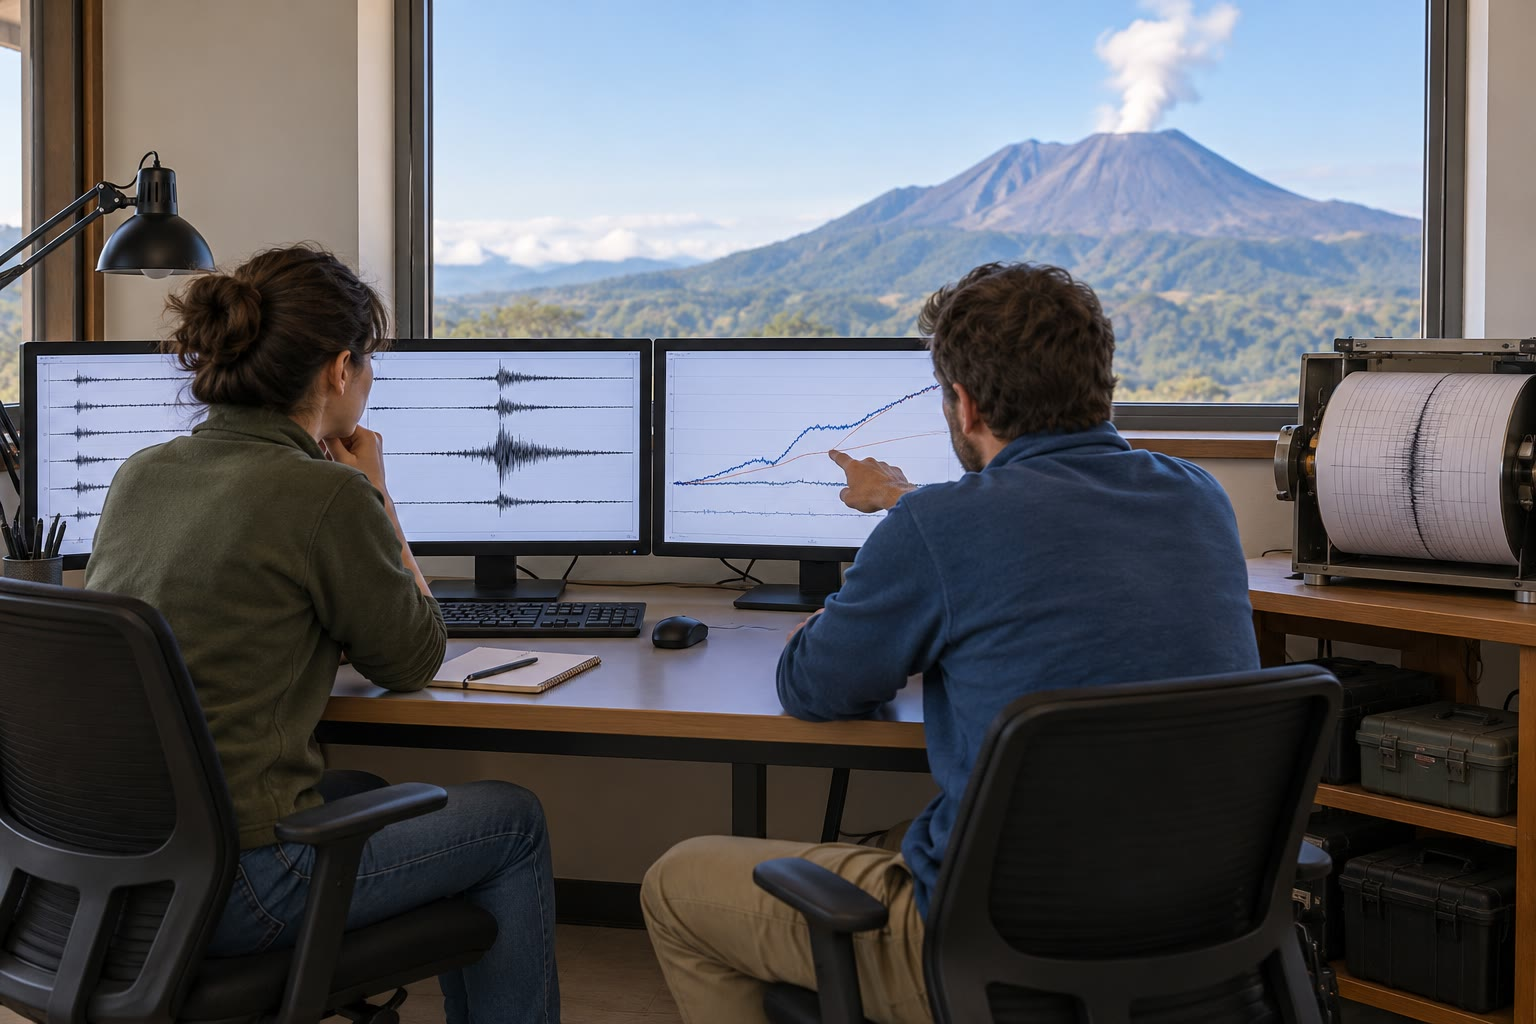
\includegraphics[width=\linewidth]{images/book4/ai/b2-volcano-observatory.jpg}
\par\smallskip{\scriptsize 科学家在火山观测站
审阅地震记录（AI 生成插图）。}
\end{minipage}
\end{inthefield}
% ledger: hvo:alert-levels

\section{练习}

\begin{exercise}[$\star$]\label{exo:b2:eruptive-styles:1}
求仅由\omterm{def:b2:eruptive-styles:tephra}{火山灰碎屑}总体积所对应的 VEI：(a) 圣海伦斯火山 1980 年 5 月 18 日的火山灰，
\qty{1.3}{km^3}；(b) 科托帕希火山第 5 层降落物，
\qty{0.29}{km^3}；(c) 一次体积为 \qty{2e6}{m^3} 的小型喷发。(d) 皮纳图博火山
1991 年喷出的物质被记为“超过 \qty{5}{km^3}”，但该次喷发被定为
VEI~6。该定级至少对应多大的总体积？
\end{exercise}
% ledger: usgs:vei-criteria, usgs:msh-1980-ash, biass19:layer5, usgs:pinatubo-1991

\begin{exercise}[$\star$]\label{exo:b2:eruptive-styles:2}
说出各\omterm{def:b2:eruptive-styles:tephra}{火山碎屑}的名称：(a) 长 \qty{0.5}{mm} 的玻屑；(b) 浮岩
碎块，直径 \qty{3}{cm}；(c) 一块棱角状的旧熔岩，直径 \qty{20}{cm}
；(d) 一个纺锤形\omterm{def:b2:eruptive-styles:tephra}{火山弹}，长 \qty{8}{cm}，两端扭曲。
\end{exercise}
% ledger: nps:pyroclast-sizes

\begin{exercise}[$\star$]\label{exo:b2:eruptive-styles:3}
已知 $H = 0.304\,Q^{0.241}$（$H$ 为火山口以上的高度，$Q$ 的单位为
\unit{kg/s}）。(a) 求 $H$，分别取 $Q = \qty{e6}{kg/s}$ 与 \qty{e8}{kg/s}；
(b) 由高 \qty{35}{km} 的\omterm{def:b2:eruptive-styles:column}{喷发柱}推算所对应的质量喷发率，以及其
强度 $I = \log_{10}Q + 3$；(c) 若测得的高度
偏高 \qty{20}{\percent}，则 $Q$ 按何倍数变化？
\end{exercise}
% ledger: aubry23:fits, brown14:record

\begin{exercise}[$\star$]\label{exo:b2:eruptive-styles:4}
科托帕希火山第 5 层降落物的总体积为 \qty{0.29}{km^3}。取降落物的总体密度为
\qty{1000}{kg/m^3}，\omterm{def:b2:magma-emplacement:magma}{岩浆}的密度为 \qty{2500}{kg/m^3}，
求其致密岩当量体积、质量及
震级 $M = \log_{10}m - 7$。
\end{exercise}
% ledger: biass19:layer5, brown14:record

\begin{exercise}[$\star\star$]\label{exo:b2:eruptive-styles:5}
某降落物在 $\sqrt A = \qty{5}{km}$ 的等厚线上厚 \qty{40}{cm}，
在 $\sqrt A = \qty{15}{km}$ 的等厚线上厚 \qty{10}{cm}，厚度按单一
指数规律变薄。求 $k$、$T_0$、厚度减半距离 $\ln 2/k$、
总体积及 VEI。
\end{exercise}

\begin{exercise}[$\star\star$]\label{exo:b2:eruptive-styles:6}
(a) 证明：等厚线 $x = \sqrt A$ 以内的体积，对于厚度按
$T_0e^{-kx}$ 变薄的降落物为 $\frac{2T_0}{k^2}[1 - (1 + kx)e^{-kx}]$。(b) 求解 $(1 + u)e^{-u} =
1/2$，精确到三位有效数字，可用逐次代入法或二分法求解。(c) 对于
对于\cref{exo:b2:eruptive-styles:5}中的降落物，体积的一半位于哪条等厚线
之外？请与所绘出的最外层等厚线距火山口的距离作比较。
\end{exercise}

\begin{exercise}[$\star\star$]\label{exo:b2:eruptive-styles:7}
温度为 \qty{850}{\celsius}（\qty{1123}{K}）的流纹质\omterm{def:b2:magma-emplacement:magma}{岩浆}，含
\qty{5.0}{\percent} 的水，溶解度 $s = 0.444$（单位：百分数每
$\sqrt{\unit{MPa}}$）；熔体密度为 \qty{2300}{kg/m^3}。(a) 求其
饱和压强，以及在压强梯度
为 \qty{0.025}{MPa/m} 时达到该压强的深度。(b) 求
\qty{10}{MPa} 时的气体体积分数（设气体留在\omterm{def:b2:magma-emplacement:magma}{岩浆}中，$R = \qty{8.314}{J/(mol.K)}$，$M =
\qty{0.018015}{kg/mol}$）。(c) 为何玄武质\omterm{def:b2:magma-emplacement:magma}{岩浆}碎裂的情况少得多，
尽管在 \qty{1}{MPa} 下，含 \qty{1}{\percent} 水的封闭系统玄武质\omterm{def:b2:magma-emplacement:magma}{岩浆}
的气体所占比例将达 \qty{92}{\percent}？
\end{exercise}
% ledger: moore98:h2o, cassidy18:fragmentation, cassidy18:ascent

\begin{exercise}[$\star\star$]\label{exo:b2:eruptive-styles:8}
(a) 深度为 \qty{5}{km} 的\omterm{prop:b2:eruptive-styles:mogi}{茂木源}体积增加 \qty{e7}{m^3}，求
其上方的隆升量（$\nu = 0.25$）。(b) 另一隆起降至其最大值的一半时，
距其中心 \qty{3.8}{km}，求其源的深度。(c) 测站在水平距离
等于源深处所见的隆升量，占最大隆升量的
几分之几？
\end{exercise}
% ledger: dmodels:mogi

\begin{exercise}[$\star\star$]\label{exo:b2:eruptive-styles:9}
武尔卡诺式爆炸将岩块抛出火山口。忽略空气阻力
与火山口边缘的高度，求以 \qty{100}{m/s} 发射的岩块的最大射程，
再求以 \qty{200}{m/s} 发射的最大射程（$g = \qty{9.81}{m/s^2}$）。空气
阻力使这些射程成为上界还是下界？为何火山口周围的
弹道危险区与发射速度的平方成正比？
\end{exercise}

\begin{exercise}[$\star\star\star$]\label{exo:b2:eruptive-styles:10}
(a) 推导方法框中给出的、由两段指数函数组成的堆积物体积公式，
假设两段直线相交处厚度连续。(b) 对科托帕希火山的第 5 层落下物，拟合的两段分别为 $T = \qty{1285}{cm}\times
e^{-0.365x}$，远端段斜率 $k_2 = \qty{0.138}{km^{-1}}$，两段相交于
$X = \qty{8.56}{km}$ 处。求该堆积物的体积，以及交点之外
部分所占的
份额。
\end{exercise}
% ledger: biass19:layer5

\begin{exercise}[$\star\star\star$]\label{exo:b2:eruptive-styles:11}
(a) 利用\cref{prop:b2:eruptive-styles:plume}，喷发率乘以 100 时，喷柱高度
增为原来的几倍？与经验指数 $0.241$ 和 $0.226$ 比较。(b) 层结更强的
大气会以何种方式改变喷柱高度，
若 $N$ 增大
\qty{20}{\percent}，高度变化多少？(c) 给出测得指数可能低于
$1/4$ 的两个原因。
\end{exercise}
% ledger: aubry23:fits

\begin{exercise}[$\star\star\star$]\label{exo:b2:eruptive-styles:12}
全球目录列出了 VEI~4 级或以上、始于 1500 年至
1899 年间的喷发 132 次，1900 至 2024 年间的 95 次。(a) 求每个
时段每世纪的喷发率。(b) 若 1900 年以来的喷发率为真，则早期
喷发中被记录的比例为多少？(c) 一项针对大规模喷发的研究发现 21 次
震级为 4 至 4.9 的喷发（1500 至 1900 年间每世纪），1900 年以来为 56 次；请比较。
(d) 为什么该比例依赖于喷发的规模？
\end{exercise}
% ledger: data:b4-gvp-eruptions, brown14:record

\section{问题：解读普林尼式堆积物}

\begin{problem}[{周末问题 --- 由浮岩落下物的等厚线推断
其喷发规模、喷柱高度及此类喷发的
频率}]
\label{pb:b2:eruptive-styles:1}
一座假想火山留下了一层浮岩落下物，它来自单次\omterm{def:b2:eruptive-styles:styles}{普林尼式喷发}阶段，
该阶段持续 \qty{10}{\hour}。等厚线在去除风向拉伸后，
取其面积的平方根，结果如下：
\begin{center}
\small
\begin{tabular}{lccccc}
\hline
$\sqrt A$ (\unit{km}) & 10 & 20 & 40 & 80 & 120 \\
厚度 $T$ (\unit{cm}) & 200 & 100 & 48 & 14 & 4.0 \\
\hline
\end{tabular}
\end{center}
数据：堆积物的堆积密度 \qty{900}{kg/m^3}；\omterm{def:b2:magma-emplacement:magma}{岩浆}的
密度 \qty{2400}{kg/m^3}；由最大碎屑测得的喷柱高度
为火山口通道以上 \qty{31}{km}；对流层顶位于 \qty{16}{km} 处。取 $H =
0.304\,Q^{0.241}$ 与 $H = 0.345\,Q^{0.226}$（$H$ 以千米计，$Q$ 以
\unit{kg/s}）。

\medskip\noindent\textbf{第一部分 --- 堆积物。}
\begin{enumerate}
\item 计算各等厚线的 $\ln T$，并说明这些点在
以 $\sqrt A$ 为横坐标作图时落在两段直线上。转折点位于何处？
\item 计算近端段直线的斜率 $k_1$ 与截距 $T_0$，
该直线经过前两条等厚线。
\item 过三条远端等厚线的最小二乘直线为 $T =
\qty{167}{cm}\times e^{-0.0311\sqrt A}$。验证该直线与每条
等厚线的偏差均在 \qty{5}{\percent} 以内。
\item 求两直线相交处的 $\sqrt A$ 值。
\item 求两段的厚度减半距离 $\ln 2/k$。
\item 若堆积物处处按近端段斜率变薄，求其体积，
即应有的体积。
\item 用两段计算堆积物的总体积，并求较缓的远端段修正所贡献
的份额。
\item 若仅测绘了近端堆积物，体积会被低估多少倍？
为什么这对古老堆积物是真实存在的风险？
\end{enumerate}

\noindent\textbf{第二部分 --- 喷发的规模。}
\begin{enumerate}[resume]
\item 给出该次喷发的 VEI。
\item 计算密岩当量体积。
\item 计算喷出物质的质量。
\item 计算震级 $M = \log_{10}m - 7$。
\item 该堆积物比 1980 年圣海伦斯火山的火山灰落下物
（\qty{1.3}{km^3}）大多少倍？
\item VEI 表将该次喷发与多高的喷柱相对应，以及对应何种
喷发类型？
\end{enumerate}

\noindent\textbf{第三部分 --- 喷柱。}
\begin{enumerate}[resume]
\item 计算普林尼式阶段的平均质量喷发率，以及其
强度 $I = \log_{10}Q + 3$。
\item 计算第一经验定律预测的喷柱高度。
\item 用第二条经验定律重复上述计算。
\item 将其与由碎屑测得的 \qty{31}{km} 比较，
并考虑两条定律的离散程度。
\item 按第一条定律，\qty{31}{km} 对应的质量喷发率是多少？它与第 15 题的值相差
几倍，何种因素可能导致这一差异？
\item 喷柱是否将气体注入平流层？对气候可能产生什么影响，
关键气体是什么？
\end{enumerate}

\noindent\textbf{第四部分 --- 发生频率。}
\begin{enumerate}[resume]
\item 依据目录计数（1950 年至 2024 年 VEI $\ge 3$ 的喷发 399 次，
1900 年以来 VEI $\ge 4$ 的喷发 95 次，1800 年以来 VEI $\ge 5$ 的 22 次，
1500 年以来 VEI $\ge 6$ 的 8 次，各时段均截至 2024 年（含），求四个年均喷发率及
其对数。
\item 验证直线 $\log_{10}\lambda_v = 3.28 - 0.85\,v$ 与每个速率的偏差
均在 \qty{10}{\percent} 以内。
\item 为什么规模越大的喷发，其统计时段起点越靠前？
\item 由该直线求 VEI $\ge 5$ 喷发的速率、其平均重现期，
以及未来 10 年内至少发生一次的概率。
\item 由该直线求 VEI $\ge 7$ 喷发的速率，并将其与
公元 1000 年以来记录的两次进行比较。
\item 由该直线求 VEI $\ge 6$ 喷发的速率，以及
未来 100 年内全球至少发生一次的概率（以百分数计），
这是本题的关键数字。该结论依赖于什么假设？
\end{enumerate}
\end{problem}
